\documentclass{article}
\usepackage[utf8]{inputenc}
\usepackage{xcolor}
\usepackage{amsmath}
\usepackage{graphicx}
\usepackage{float}
\usepackage{minted}
\usepackage{circuitikz}
\usepackage{tikz}
\usetikzlibrary{shapes, arrows, calc, positioning, circuits.logic.US, circuits.logic.IEC}
\usepackage{geometry}
\geometry{a4paper, margin=1in}
\usepackage{hyperref}
\usemintedstyle{trac}

\usepackage{fancyhdr}
\pagestyle{fancy}
\fancyhf{}
\renewcommand{\headrulewidth}{0pt}
\fancyfoot[C]{\small 010153101 Digital Circuit and Microprocessor Fundamental}
\fancyfoot[R]{\thepage}

% Redefine plain style to match fancy style (for the title page)
\fancypagestyle{plain}{%
  \fancyhf{}%
  \fancyfoot[C]{\small 010153101 Digital Circuit and Microprocessor Fundamental}%
  \fancyfoot[R]{\thepage}%
  \renewcommand{\headrulewidth}{0pt}%
}

\title{Laboratory Exercise 2 \\ Logic Optimization, Universal Gates and Parity}
\author{}
\date{}

\begin{document}

\maketitle

\section*{Introduction}
This laboratory exercise accompanies Lecture 3 (Logic Optimization using Karnaugh Maps). You will minimize a logic function with a Karnaugh map, implement it with NAND gates only (a two-level NAND-NAND circuit), take advantage of ``don't-care'' conditions, and finally design a parity generator and checker with exclusive-OR gates in Quartus. As in Labs 0 and 1, no VHDL is needed. The session is two hours long, so the paper work is done in the pre-lab.

\section*{Objectives}
\begin{enumerate}
    \item To simplify a four-variable Boolean function using a Karnaugh map.
    \item To implement a Sum-of-Products function using only NAND gates and to verify it on the breadboard.
    \item To see how don't-care conditions reduce the size of a circuit.
    \item To design a parity generator and a parity checker and to detect a single-bit error.
\end{enumerate}

\section*{Equipment Required}
\begin{itemize}
    \item DC Power Supply (+5V), Digital Multimeter
    \item Breadboard and Jumper Wires
    \item TTL ICs: 74LS00 (Quad 2-Input NAND) $\times 2$, 74LS04 (Hex Inverter)
    \item Resistors: $330\Omega$ (for LEDs and pull-down)
    \item DIP switches, LEDs (Red/Green)
    \item Intel DE0-CV board and a PC with Quartus Prime
    \item (Optional) Logisim or Logisim-evolution: a light-weight tool for drawing and simulating small circuits at home or in the laboratory. It cannot program the DE0-CV board, so Quartus Prime is still needed for the board.
\end{itemize}

\section*{Pre-lab (complete before the session)}
Complete Part I(a)--(d), Part II(a)--(b) and Part III(a) \emph{before} the laboratory session. The pin numbers of the 74LS00 and 74LS04 are the same as in Lab 1 (Table 1 of that sheet). You can check your K-maps, expressions and NAND-NAND drawing in \textbf{Logisim} (Combinational Analysis window for the minimized SOP of a truth table). Remember to use the \textbf{LED indicator stage} (inverter + LED + $330\,\Omega$) for each output that you observe on the breadboard.

\section*{Part I: Two-Level NAND-NAND Implementation (about 45 min)}

Consider the function
\[ F(A,B,C,D) = \sum m(0,1,2,5,8,9,10,13). \]

\subsection*{Simplify with a K-map}
\begin{enumerate}
    \item[(a)] Fill the K-map of Figure \ref{fig:kmap1} with the values of $F$.
    \item[(b)] Circle the groups of 1s so that each group is as large as possible and the \emph{minimum number of groups} covers all 1s. Is there any prime implicant that is not needed? \underline{\hspace{4cm}}
    \item[(c)] Write the minimized SOP expression: $F = $ \underline{\hspace{8cm}}
\end{enumerate}

\begin{figure}[H]
    \centering
    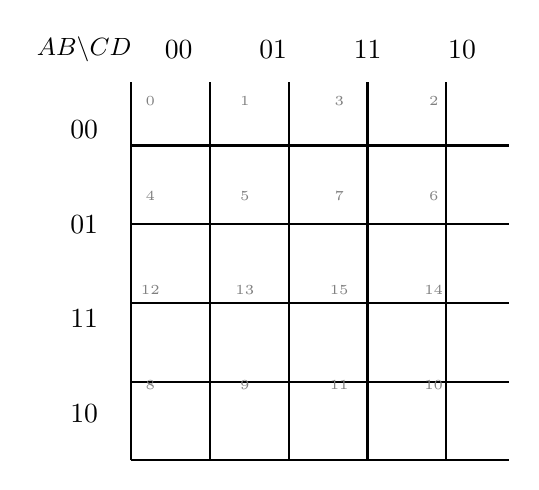
\begin{tikzpicture}[x=1.2cm,y=1.2cm]
        \draw[thick] (0,0) grid (4,4);
        % column labels (CD)
        \foreach \i/\l in {0/00,1/01,2/11,3/10} {\node at (\i+0.5,4.35) {\l};}
        % row labels (AB)
        \foreach \i/\l in {0/00,1/01,2/11,3/10} {\node at (-0.5,3.5-\i) {\l};}
        \node at (-0.5,4.35) {\small $AB\backslash CD$};
        % minterm numbers in each cell
        \foreach \r/\c/\m in {0/0/0,0/1/1,0/2/3,0/3/2,
                              1/0/4,1/1/5,1/2/7,1/3/6,
                              2/0/12,2/1/13,2/2/15,2/3/14,
                              3/0/8,3/1/9,3/2/11,3/3/10}
            {\node[gray,font=\tiny] at (\c+0.2,3.8-\r) {\m};}
    \end{tikzpicture}
    \caption{K-map for $F(A,B,C,D)$ (the small numbers are the minterm indices; write 0 or 1 in each cell).}
    \label{fig:kmap1}
\end{figure}

\subsection*{Convert to NAND-NAND form}
An SOP expression becomes a NAND-NAND circuit when every AND and the final OR are replaced with NAND gates (Lecture 3, De Morgan's theorem):
\[ F = P_1 + P_2 = \big( (P_1)' \cdot (P_2)' \big)' \]
An inverter can be made from a NAND gate by connecting its two inputs together.

\begin{enumerate}
    \item[(d)] \textbf{(Pre-lab)} Draw the NAND-NAND circuit of your expression. Complemented inputs ($B'$, $C'$, $D'$) must also be built from NAND gates. How many 2-input NAND gates and how many 74LS00 ICs do you need? \underline{\hspace{4cm}}
    \item[(e)] Build the circuit on the breadboard, with $A, B, C, D$ taken from four switches and $F$ displayed by an LED indicator stage.
    \item[(f)] Test all 16 input combinations and complete Table \ref{tab:kmap_test}.
\end{enumerate}

\begin{table}[H]
    \centering
    \small
    \setlength{\tabcolsep}{4pt}
    \begin{tabular}{|c|cccc|c|c||c|cccc|c|c|}
        \hline
        $m$ & $A$ & $B$ & $C$ & $D$ & Exp. & Meas. & $m$ & $A$ & $B$ & $C$ & $D$ & Exp. & Meas. \\
        \hline
        0 & 0&0&0&0 & 1 & & 8 & 1&0&0&0 & 1 & \\
        1 & 0&0&0&1 & 1 & & 9 & 1&0&0&1 & 1 & \\
        2 & 0&0&1&0 & 1 & & 10 & 1&0&1&0 & 1 & \\
        3 & 0&0&1&1 & 0 & & 11 & 1&0&1&1 & 0 & \\
        4 & 0&1&0&0 & 0 & & 12 & 1&1&0&0 & 0 & \\
        5 & 0&1&0&1 & 1 & & 13 & 1&1&0&1 & 1 & \\
        6 & 0&1&1&0 & 0 & & 14 & 1&1&1&0 & 0 & \\
        7 & 0&1&1&1 & 0 & & 15 & 1&1&1&1 & 0 & \\
        \hline
    \end{tabular}
    \caption{Test of the NAND-NAND circuit (Exp. = expected value of $F$, Meas. = LED reading).}
    \label{tab:kmap_test}
\end{table}

\section*{Part II: Don't-Care Conditions (about 30 min)}

A BCD digit uses the 4-bit codes $0000$ to $1001$ ($0$ to $9$). The codes $1010$ to $1111$ never occur in a BCD system, so the output of the circuit for those inputs is a \textbf{don't care}. A BCD ``prime-number detector'' has an output $P$ that is 1 when the BCD digit is a prime number ($2, 3, 5$ or $7$).

\begin{enumerate}
    \item[(a)] Fill in the K-map of Figure \ref{fig:kmap2} for $P$, marking the unused codes with an \textbf{X}.
    \item[(b)] Simplify $P$ twice: first \emph{treating all X as 0}, then \emph{using the X's wherever they make a group larger}. \\[0.2cm]
    $P_{\text{no DC}} = $ \underline{\hspace{6cm}} \\[0.2cm]
    $P_{\text{DC}} = $ \underline{\hspace{6cm}}
    \item[(c)] Create a new Quartus project \texttt{lab2}. Draw both circuits in the Block Editor with the same inputs $A, B, C, D$ (BCD digit, $A$ is the MSB). (The comparison of parts (c)--(e) can also be done in Logisim; the board test of (f) needs Quartus.)
    \item[(d)] Simulate with a waveform file that counts from $0000$ to $1111$. Compare the outputs. For which input codes do they differ? Does this matter in a BCD system?
    \item[(e)] Compile the project. Which circuit is smaller (number of gates)? \underline{\hspace{4cm}}
    \item[(f)] Implement $P_{\text{DC}}$ on the DE0-CV board with SW3--SW0 as $A$--$D$ and LEDR0 as $P$. Step through the digits $0$ to $9$ with the switches and verify that $P$ is lit for $2, 3, 5, 7$ only.
\end{enumerate}

\begin{figure}[H]
    \centering
    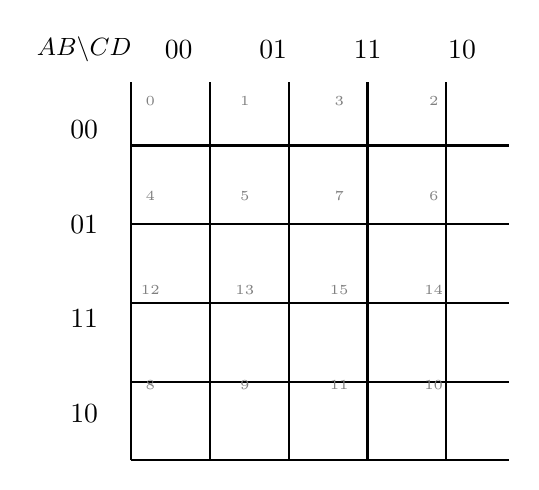
\begin{tikzpicture}[x=1.2cm,y=1.2cm]
        \draw[thick] (0,0) grid (4,4);
        \foreach \i/\l in {0/00,1/01,2/11,3/10} {\node at (\i+0.5,4.35) {\l};}
        \foreach \i/\l in {0/00,1/01,2/11,3/10} {\node at (-0.5,3.5-\i) {\l};}
        \node at (-0.5,4.35) {\small $AB\backslash CD$};
        \foreach \r/\c/\m in {0/0/0,0/1/1,0/2/3,0/3/2,
                              1/0/4,1/1/5,1/2/7,1/3/6,
                              2/0/12,2/1/13,2/2/15,2/3/14,
                              3/0/8,3/1/9,3/2/11,3/3/10}
            {\node[gray,font=\tiny] at (\c+0.2,3.8-\r) {\m};}
    \end{tikzpicture}
    \caption{K-map for the BCD prime-number detector $P$.}
    \label{fig:kmap2}
\end{figure}

\section*{Part III: Parity Generator and Checker (about 25 min)}

When data are transmitted or stored, a single bit may be flipped by noise. An \textbf{even-parity} bit $P$ is added to the data so that the total number of 1s in (data + $P$) is even. The receiver recomputes the parity; if the result is 1, an error is detected. Figure \ref{fig:parity} shows a system for 3 data bits $D_2 D_1 D_0$.

\begin{figure}[H]
    \centering
    \begin{circuitikz}[circuitikz/logic ports=ieee, scale=0.9, transform shape]
        % parity generator
        \draw (0,0) node[xor port] (g1) {};
        \draw (3.2,-0.8) node[xor port] (g2) {};
        \draw (g1.in 1) -- ++(-1,0) node[left] {$D_2$};
        \draw (g1.in 2) -- ++(-1,0) node[left] {$D_1$};
        \draw (g1.out) -- ++(0.4,0) |- (g2.in 1);
        \draw (g2.in 2) -- ++(-3.6,0) node[left] {$D_0$};
        \draw (g2.in 2) ++(-3.0,0) coordinate (jD0);
        \fill (jD0) circle (1.5pt);
        \draw (g2.out) -- ++(0.8,0) coordinate (Pn) node[above] {$P$};
        \fill (Pn) circle (1.5pt);
        % error injection
        \draw (3.2,-2.9) node[xor port] (e) {};
        \draw (jD0) |- (e.in 1);
        \draw (e.in 2) -- ++(-1.8,0) node[left] {$ERR$};
        \draw (e.out) -- ++(0.8,0) coordinate (Dn) node[below] {$D_0'$};
        % checker block
        \node[draw, minimum width=3cm, minimum height=2.0cm, align=center] (chk) at (9,-1.4) {Parity checker\\(3 XOR gates)};
        \draw (chk.west) ++(0,0.6) -- ++(-0.8,0) node[left] {$D_2$};
        \draw (chk.west) ++(0,0.2) -- ++(-0.8,0) node[left] {$D_1$};
        \draw (Pn) |- ($(chk.west)+(0,-0.2)$);
        \draw (Dn) |- ($(chk.west)+(0,-0.6)$);
        \draw (chk.east) -- ++(0.9,0) node[right] {$E$};
    \end{circuitikz}
    \caption{Parity system: generator, error-injection XOR ($ERR=1$ flips $D_0$) and checker.}
    \label{fig:parity}
\end{figure}

\begin{enumerate}
    \item[(a)] \textbf{(Pre-lab)} Write the Boolean expression of the even-parity bit: $P = $ \underline{\hspace{5cm}} and of the error flag $E$ (using $D_2, D_1, D_0', P$): $E = $ \underline{\hspace{5cm}}
    \item[(b)] In the Quartus project (or in Logisim), draw the whole system of Figure \ref{fig:parity} as a schematic with XOR gates (6 gates), inputs $D_2, D_1, D_0, ERR$ and outputs $P$ and $E$.
    \item[(c)] Simulate: apply the 8 data combinations first with $ERR=0$ and then with $ERR=1$, and complete Table \ref{tab:parity}.
    \item[(d)] Assign $D_2, D_1, D_0, ERR$ to SW3--SW0, $P$ to LEDR1 and $E$ to LEDR0 and download the circuit to the board. Check a few rows of Table \ref{tab:parity} on the board.
    \item[(e)] What kind of errors can this system detect? What kind can it \emph{not} detect?
\end{enumerate}

\begin{table}[H]
    \centering
    \begin{tabular}{|c|c|c|c|c|c|c|c|}
        \hline
        $D_2$ & $D_1$ & $D_0$ & $P$ expected & $P$ (sim.) & $E$ ($ERR=0$) & $E$ ($ERR=1$) \\
        \hline
        0 & 0 & 0 & 0 & & & \\
        0 & 0 & 1 & 1 & & & \\
        0 & 1 & 0 & & & & \\
        0 & 1 & 1 & & & & \\
        1 & 0 & 0 & & & & \\
        1 & 0 & 1 & & & & \\
        1 & 1 & 0 & & & & \\
        1 & 1 & 1 & & & & \\
        \hline
    \end{tabular}
    \caption{Parity generator and checker results.}
    \label{tab:parity}
\end{table}

\section*{Extension (take-home, or if time permits)}
\begin{enumerate}
    \item Compare the cost of your minimized circuit of Part I with a direct implementation of the canonical SOP (eight 4-input AND terms and one 8-input OR). How many gate inputs have you saved?
    \item Obtain a Product-of-Sums expression for $F$ by grouping the 0s of the K-map and show that it is equal to your SOP expression.
    \item Build the parity generator and checker of Part III on the breadboard with two 74LS86 ICs (6 XOR gates) and test it with Table \ref{tab:parity}.
\end{enumerate}

\section*{Check-off}
Show your instructor or teaching assistant:
\begin{enumerate}
    \item Your K-map, minimized expression and NAND-NAND circuit working on the breadboard (Table \ref{tab:kmap_test}).
    \item The simulation of the prime-number detector with and without don't cares.
    \item The parity system simulation and the circuit on the board (Table \ref{tab:parity}).
\end{enumerate}

\vspace{1cm}
\noindent \textbf{Updated By:} R. Sutthaweekul \\
\textbf{Version:} 1.0 \\
\textbf{Release Date:} 2026-11-11

\end{document}
